 \fancyhead[LO,CE]{Chapter: \thechapter| Réalisation}
\section{Introduction}
Une fois la conception validée, il est temps de passer à la réalisation. Nous présentons dans ce chapitre le module réalisé en utilisant des captures d’écran  pour montrer ses principales fonctionnalités. Nous commençons par présenter les outils et les technologies utilisées pour le développement, ensuite nous présenterons l’architecture technique de la solution et l’architecture des codes.

\section{Outils et Technologies utilisées pour le développement}
Pour le développement,  nous avons utilisé : 

   
   \comment{
    \subsection{Architecture Modèle/Vue/Contrôleur (MVC)}


Pour d'organiser  l'interface graphique Nous avons utiliser l'architecture Modèle/Vue/Contrôleur (MVC).  Elle consiste à distinguer trois entités distinctes qui sont, le modèle, la vue et le contrôleur ayant chacun un rôle précis dans l'interface. \parencite{mvc}

\begin{itemize}
	\item 	\textbf{modèle :} données (accès et mise à jour)
	\item 	\textbf{vue :} interface utilisateur (entrées et sorties)
	\item 	\textbf{contrôleur :} gestion des événements et synchronisation
\end{itemize}


\begin{figure}[H]
	\centering
	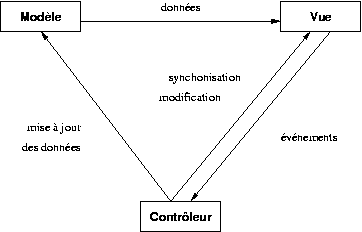
\includegraphics[width=0.6\linewidth]{images/mvc}
	\caption{Interactions entre le modèle, la vue et le contrôleur \parencite{mvc}}
	\label{fig:mvc}
\end{figure}
}
\subsection{Technologies web } 
\subsubsection{Technologies web (HTML5, JS et CSS3):} 
\begin{itemize}
	
 \item  \textbf{HTML5 (Hypertext Markup Language 5) :} c’est un language de balisage permettant de décrire la structure et le contenu des pages Web. 
 
 \item \textbf{JS (JavaScript) :} c’est un langage de script orienté objet utilisé pour dynamiser les pages Web et permettre une interaction avec l’utilisateur. Il est exécuté au niveau du navigateur. 
 
 \item \textbf{CSS3 (Cascading Style Sheets) :} c’est un langage permettant de gérer la présentation et la mise en forme des pages web. (Positionnement des éléments, couleurs, tailles et polices, etc…). 
 
 

 \subitem  \authorimg{Bootstarp}  \textbf{Le Framework Bootstrap } 
 Nous avons utilisé le Framework CSS \textbf{Bootstrap3} qui dispose d’une grid pour faciliter la gestion de la mise en forme des pages HTML. Il offre aussi des composants de design basés sur HTML et CSS avec un\textbf{ Responsive design} (voir la figure \ref{fig:responsive}) qui permet un affichage qui s’adapte à la taille de l’écran, que ce soit une tablette, un smartphone ou un ordinateur. 
 
 
\begin{figure}[H]
	\centering
	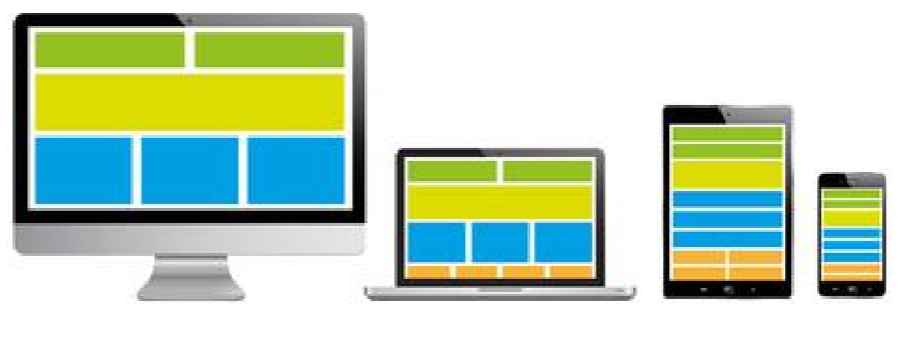
\includegraphics[width=0.5\linewidth]{images/responsive}
	\caption{Responsive design }
	\label{fig:responsive}
\end{figure}
\end{itemize}

 \subsubsection{Thymeleaf}

Nous avons utilisé Thymeleaf comme un moteur de template Java pour le traitement et la création de HTML, XML, JavaScript, CSS et du texte.

La bibliothèque est extrêmement extensible et sa capacité naturelle de gabarit permet aux prototypes de prototyper des gabarits, ce qui rend le développement très rapide par rapport aux autres moteurs de gabarits populaires tels que JSP.

 \subsection{  Workflow :}
Pour l'implémentation de Workflow nous avons utilisé: 
\begin{itemize}
	\item bpmn js
	\item Camunda BPM
\end{itemize}

\subsubsection{bpmn js} 
bpmn-js est une boîte à outils de rendu et un modélisateur Web BPMN 2.0. pour la modélisation de flux de travaux "Workflow" Il est écrit en JavaScript, intègre les diagrammes BPMN 2.0 dans les navigateurs modernes et ne requiert aucun serveur. Cela facilite son intégration dans n’importe quelle application Web.



\subsubsection{ Camunda BPM}
Nous avons utilisé Camunda BPM car est un système de gestion de flux de travaux gratuit écrit en Java qui définit et exécute les processus métier dans BPMN 2.0. 


 \subsection{Spring}
 
  \subsubsection{Spring Framework }
  
  
  Spring Framework fournit un modèle complet de programmation et de configuration pour les applications d'entreprise modernes basées sur Java - sur tout type de plate-forme de déploiement.
   
 
  Un élément clé de Spring est le support infrastructurel au niveau de l’application: Spring met l’accent sur la «plomberie» des applications d’entreprise afin que les équipes puissent se concentrer sur la logique métier au niveau de l’application, sans liens inutiles avec des environnements de déploiement spécifiques.
  
 \subsubsection{Spring boot}
Nous avons utilisé Spring Boot pour  facilite la création d'applications basées sur Spring autonomes et de niveau production que vous pouvez "exécuter".
 
  
   \subsubsection{Spring Data}
   La mission de Spring Data est de fournir un modèle de programmation familier et cohérent, basé sur Spring, pour l’accès aux données tout en conservant les caractéristiques spéciales du magasin de données sous-jacent.
   
   Il facilite l'utilisation des technologies d'accès aux données, des bases de données relationnelles et non relationnelles, des infrastructures de réduction de carte et des services de données en nuage. Il s'agit d'un projet parapluie contenant de nombreux sous-projets spécifiques à une base de données donnée.
   
   \subsubsection{Spring Security}
  Pour la parti de sécurité  nous avons utilisé  \textbf{Spring Security} car  est un cadre d’authentification et de contrôle d’accès puissant et hautement personnalisable. C'est la norme de facto pour la sécurisation des applications basées sur Spring.
   
   Spring Security est une infrastructure qui fournit à la fois l’authentification et l’autorisation aux applications Java. Comme tous les projets Spring, la véritable force de Spring Security réside dans la facilité avec laquelle elle peut être étendue pour répondre aux exigences personnalisées.
 \subsubsection{Spring Cloud}
 Spring Cloud fournit aux développeurs des outils permettant de créer rapidement certains modèles courants dans les systèmes distribués (gestion de la configuration, découverte de services, disjoncteurs, routage intelligent, micro-proxy, bus de contrôle, jetons à usage unique, verrous globaux, élection des dirigeants, distribution sessions, état du cluster). La coordination des systèmes distribués conduit à des modèles de plaque de chaudière et, grâce à Spring Cloud, les développeurs peuvent rapidement mettre en service des services et des applications mettant en œuvre ces modèles. Ils fonctionneront bien dans n’importe quel environnement distribué, y compris l’ordinateur portable du développeur, les centres de données à nu et les plateformes gérées telles que Cloud Foundry\footnote[1]{\samepage Cloud Foundry facilite, accélère et simplifie la création, le test, le déploiement et la mise à l'échelle des applications, en offrant un choix de clouds, de cadres de développement et de services d'application. Il s'agit d'un projet open source, disponible via une variété de distributions de cloud privé et d'instances de cloud public.}.
 
 
  \subsubsection{Spring Cloud Netflix}
 Spring Cloud Netflix fournit des intégrations Netflix OSS pour les applications Spring Boot via la configuration automatique et la liaison à Spring Environment et à d'autres idiomes de modèles de programmation Spring. Quelques annotations simples vous permettent d'activer et de configurer rapidement les modèles courants dans votre application et de créer de grands systèmes distribués avec des composants Netflix testés au combat. Les modèles fournis incluent la découverte de service (Eureka), le disjoncteur (Hystrix), le routage intelligent (Zuul) et l’équilibrage de la charge côté client (ruban).
 
 \subsection{   Micro Service }

 L'objectif principal de la mise en œuvre des micro-services est de scinder l'application en un service distinct pour chaque fonctionnalité de base et chaque service de l'API. Elle devrait être déployée indépendamment sur le cloud. Nous avons choisi le langage de programmation réactif du projet familial spring.io avec un ensemble de composants pouvant être utilisés pour mettre en œuvre notre modèle d'exploitation. Spring Cloud intègre très bien les composants Netflix dans l’environnement Spring. Il utilise une configuration automatique et une convention de configuration similaire à celle du fonctionnement de Spring Boot.


\subsubsection{Pourquoi l’architecture de Microservices?}

Nous avons choisi l'architecture de micro-services pour écrire chaque fonctionnalité en tant que service distinct pour les fonctionnalités de base et d'API, ce qui nous aide à réaliser la livraison et l'intégration en continu.

\subsubsection{Patterns dans l'architecture des microservices}



\begin{itemize}
\item  \textbf{Api Gatway }


\begin{enumerate}
	
\item 	  Choisissez de créer l’application en tant qu’ensemble de micro-services.

\item	  Décidez comment le client de l'application va interagir avec les micro-services.

\item	  Avec une application monolithique, il n'y a qu'un seul ensemble de points d'extrémité (généralement répliqués, à charge équilibrée).

\item	  Dans une architecture de micro-services, chaque micro-service expose cependant un ensemble de
points finaux.
\end{enumerate}


\item \textbf{Service registry}

\begin{enumerate}
\item 	  Le registre de service aide à déterminer l’emplacement des instances de service pour envoyer la demande au correspondant
	un service
	
\item 	  Ici, nous avons utilisé Netflix Eureka pour enregistrer un service pouvant être enregistré dans le registre de services.
	serveur et il peut être identifié par le routeur.

	
\end{enumerate}
\item \textbf{Service Discovry}
\begin{enumerate}


\item   Dans une application monolithique, les services s'appellent par le biais d'appels de méthode ou de procédure au niveau de la langue.

\item   Toutefois, dans une application moderne basée sur des micro-services, elle s'exécute généralement dans des environnements virtualisés où le nombre
des instances d'un service et de leurs emplacements change de façon dynamique.

\item   Chaque service peut être identifié à l'aide d'un routeur enregistré auprès du serveur de registre de services.
	
\end{enumerate}
\end{itemize}



\subsubsection{Architecture des microservices via les composants Netflix}
Nous avons utilisé les composants Netflix pour réaliser les modèles d’architecture de microservices ci-dessus. \parencite{MicroServices}.

% Please add the following required packages to your document preamble:
% \usepackage[table,xcdraw]{xcolor}
% If you use beamer only pass "xcolor=table" option, i.e. \documentclass[xcolor=table]{beamer}
% \usepackage[normalem]{ulem}
% \useunder{\uline}{\ul}{}
\begin{table}[H]
	\begin{tabular}{|l|l|}
		\hline
	  \textbf{Operations Component}  & \textbf{Spring, Netflix OSS } \\ \hline
		Service Discovery server & Netflix Eureka \\ \hline
		Edge Server & Netflix Zuul \\ \hline
		Central configuration server & Spring Cloud Config Server \\ \hline
		Dynamic Routing and Load Balancer & Netflix Ribbon \\ \hline
		OAuth 2.0 protected API’s & Spring Cloud + Spring Security OAuth2 \\ \hline
		Monitoring & Netflix Hystrix dashboard and turbine \\ \hline
	\end{tabular}
 \label{fig:Netflix}
\caption{Architecture des microservices via les composants Netflix \parencite{MicroServices}}
\end{table}

\subsection{Composantes majeures de Netflix}



\subsubsection{Service Discovery Server} 

\authorimg{images/ms-img04} Netflix Eureka permet aux micro-services de s’enregistrer eux-mêmes au moment de leur exécution, tels qu’ils apparaissent dans la structure du système.
\parencite{MicroServices}


\subsubsection{Routage dynamique et équilibreur de charge} 

\authorimg{images/ms-img05}  Netflix Ribbon peut être utilisé par les consommateurs de services pour rechercher des services au moment de l’exécution. Le ruban utilise les informations disponibles dans Eureka pour localiser les instances de service appropriées. Si plusieurs instances sont trouvées, le Ruban appliquera un équilibrage de charge pour répartir les demandes sur les instances disponibles. Le ruban ne s'exécute pas en tant que service distinct, mais en tant que composant intégré dans chaque consommateur de service.\parencite{MicroServices}





\subsubsection{Serveur Edge} 

\authorimg{images/ms-img06}  Zuul est (bien sûr) notre gardien du monde extérieur, ne permettant pas le passage de demandes externes non autorisées. Zulu fournit également un point d'entrée bien connu aux micro-services dans le paysage système. L'utilisation de ports alloués de manière dynamique est pratique pour éviter les conflits de ports et minimiser l'administration, mais elle rend évidemment la tâche plus difficile pour tout consommateur de services donné. Zuul utilise Ribbon pour rechercher les services disponibles et achemine la demande externe vers une instance de service appropriée.\parencite{MicroServices}


\subsection{Spring Boot et Spring Cloud Netflix OSS – Micro Service Architecture}

\subsubsection{Micro Services avec Spring Boot}

 

Spring Boot est un  nouveau framework de l'équipe de Pivotal, conçu pour simplifier le démarrage et le développement d'une nouvelle application Spring. Le cadre adopte une approche de configuration avisée, libérant les développeurs de la nécessité de définir la configuration standard.\parencite{MicroServices}

\subsubsection{Spring Cloud Netflix}
 

Spring cloud Netflix fournit des intégrations Netflix OSS pour les applications de démarrage printanier via la configuration automatique et la liaison à l'environnement Spring et à d'autres modèles de programmation Spring. Avec quelques annotations simples, nous pouvons rapidement activer et configurer des modèles courants dans une application et construire des systèmes distribués volumineux avec des composants Netflix. De nombreuses fonctionnalités sont disponibles avec le nuage de printemps Netflix. Ici, nous avons répertorié certaines des fonctionnalités communes que nous avons implémentées avec les micro-services avec Spring Boot et Netflix, \parencite{MicroServices}

\begin{itemize}
\item \textbf{Découverte du service:}
	
	Les instances Eureka peuvent être enregistrées et les clients peuvent
	Découvrez les exemples à l'aide de haricots à gestion printanière
	

\item \textbf{	Création de service:}	
	Le serveur Eureka intégré peut être créé avec
	configuration Java déclarative
	
\item \textbf{	Configuration Externel:}	
	
	Bridge from the Spring Environment (permet aux utilisateurs de
	configuration des composants Netflix à l'aide de Spring Boot
	conventions)
	
      \item \textbf{	Routeur et filtre:}	
	
	Enregistrement automatique des filtres Zuul, et un simple
	convention sur l'approche de configuration pour la création de proxy inverse.
\end{itemize}


\subsection{Maven} 
 


Maven est essentiellement un outil de gestion et de compréhension de projet. 

Maven offre des fonctionnalités de :
\begin{itemize}
\item  Construction,  Compilation ;
\item  Documentation ;
\item  Rapport ;
\item  Gestion des dépendances ;
\item  Gestion des sources ;
\item  Mise à jour de projet ;
\item  Déploiement.
\end{itemize}

\subsubsection{ POM  }
Le \textbf{POM} (\textbf{P}roject \textbf{O}bject \textbf{M}odel) est une façon de décrire, de manière déclarative, un projet au sens de Maven. Cette description est contenue dans le fichier \textbf{pom.xml} présent dans le repertoire de base du projet. Le fichier pom.xml contient donc tous les éléments permettant de gérer le cycle de vie du projet. \parencite{maven}.

\textbf{\underline{Code xml :}}	\\

 \lstset{language=XML}
\begin{lstlisting}

<project xmlns="http://maven.apache.org/POM/4.0.0" xmlns:xsi="http://
www.w3.org/2001/XMLSchema-instance" xsi:schemaLocation="http://maven.
apache.org/POM/4.0.0 http://maven.apache.org/maven-v4_0_0.xsd"> 

<modelVersion>4.0.0</modelVersion> 
<groupId>com.mycompany.app</groupId> 
<artifactId>my-app</artifactId> 
<packaging>jar</packaging> 
<version>1.0-SNAPSHOT</version> 
<name>Maven Quick Start Archetype</name> 
<url>http://maven.apache.org</url> 

<dependencies> 
<dependency> 
<groupId>junit</groupId> 
<artifactId>junit</artifactId> 
<version>3.8.1</version> 
<scope>test</scope> 
</dependency> 
</dependencies> 

</project>

\end{lstlisting}

\begin{itemize}

\item \textbf{Project} : c'est la balise racine de tous les fichiers pom.xml.
\item \textbf{ModelVersion} : cette balise indique la version de POM utilisée. Bien que cette version ne change pas fréquemment, elle est obligatoire afin de garantir la stabilité d'utilisation.
\item \textbf{GroupId} : cette balise permet d'identifier un groupe qui a créé le projet. Cette clé permet d'organiser et de retrouver plus facilement et rapidement le projet.
\item \textbf{ArtifactId} : cette balise indique un nom unique utilisé pour nommer les artifacts à construire.
\item \textbf{Packaging} : type de packaging du projet ( ex. : JAR, WAR, EAR, etc.).
version : version de l'artifact généré par le projet.
\item \textbf{Name} : nom du projet.
\item \textbf{Url} : adresse du site du projet.
description : description du projet.
\item \textbf{Dependencies} : balise permettant de gérer les dépendances.
\end{itemize}

\subsubsection{Archetype }
Un archetype est un template de projet. Le fait d'utiliser des archetypes pour initialiser un projet permet de gagner du temps et de respecter une certaine convention. \parencite{maven}.

\subsubsection{Dépendance  }
 Une dépendance est une référence vers un artefact spécifique contenu dans un repository. Cet artefact est nécessaire pour une ou plusieurs phases du cycle de vie du projet. \parencite{maven}.
 
 L'exemple le plus simple est une dépendance sur une bibliothèque jar qui permet d'en utiliser le contenu dans le projet.\parencite{maven}.
 
 \subsubsection{Artefact }
 
 Dans Maven, un artefact est un élément spécifique issu de la construction du logiciel. 
 
 Dans Java, les artefacts les plus communs sont des JARs, mais ce peut être aussi un fichier WAR, un EAR, un ZIP, etc.\parencite{maven}.

  
 
     \subsubsection{Le groupId/artifactId }
   Le groupId est l'identifiant du groupe, à l'origine du projet. GroupId suit les mêmes règles de nommage que les packages  Java (exemple : fr.masociete.monprojet), et on choisit généralement comme groupId le nom du top package du projet. \parencite{maven}.
   
   L'artifactId est l'identifiant du projet au sein de ce groupe. 
   
   L'artifactId est utilisé par défaut pour construire le nom de l'artefact final (exemple : pour un artifactId=monprojet, le nom du fichier jar généré sera monprojet-version.jar).  \subsubsection{  SNAPSHOT  }
 
    Par convention, une version en cours de développement d'un projet voit son numéro de version suivi d'un -SNAPSHOT. 
    
    Ainsi un projet en version 2.0-SNAPSHOT signifie que cette version est une pré-version de la version 2.0, en cours de développement. 
    
    Ce concept de SNAPSHOT est particulièrement important pour Maven. En effet, dans la gestion des dépendances, Maven va chercher à mettre à jour les versions SNAPSHOT régulièrement pour prendre en compte les derniers développements. 
    
    L'utilisation d'une version SNAPSHOT permet de bénéficier des dernières fonctionnalités d'un projet, mais en contrepartie, cette version peut être (et est) appelée à être modifiée de façon importante, sans aucun préavis. \parencite{maven}.
       \subsubsection{Le repository local et distant }
    Un repository local est un répertoire sur le poste du développeur permettant de stocker, suivant la même arborescence, tous les artefacts téléchargés depuis le(s) repository distant(s). \parencite{maven}. 
    
     Un projet ayant pour POM :
     
     \textbf{\underline{Code xml :}}\\
    \lstset{language=XML}
\begin{lstlisting}
<project>
<modelVersion>4.0.0</modelVersion>
<groupId>fr.masociete</groupId>
<artifactId>monprojet</artifactId>
<version>1.0</version>
</project>
\end{lstlisting}
     
\section{Création d'un service cloud par spring et micro service :}

\subsection{Outils et Versions}

\begin{itemize}
\item Spring Boot Version: 2.0.1
\item Spring Cloud Version 1.2.4
\item Java Version 1.8.0 
\item Maven Version 3.6.1
\item  Tu peux utiliser l'éditeur eclipse STS ou IntelliJ IDEA ( votre choix ).
\end{itemize}



Nous allons donc créer les microservices suivants:
\subsubsection{Service principal:} Service principal, qui offre par exemple une API REST pour  la liste des utilisateurs du système.   (voir la Figure \ref{fig:class01} dans le chapitre 2 qui représente le diagramme de classe).
	
\subsubsection{Config Service :} Service de configuration, dont le rôle est de centraliser les fichiers de configuration des différents microservices dans un endroit unique.
	
\subsubsection{Proxy Service :} Passerelle se chargeant du routage d'une requête vers l'une des instances d'un service, de manière à gérer automatiquement la distribution de charge.
	
\subsubsection{Discovery Service:} Service permettant l'enregistrement des instances de services en vue d'être découvertes par d'autres services.
 




\begin{figure}[H]
	\centering
	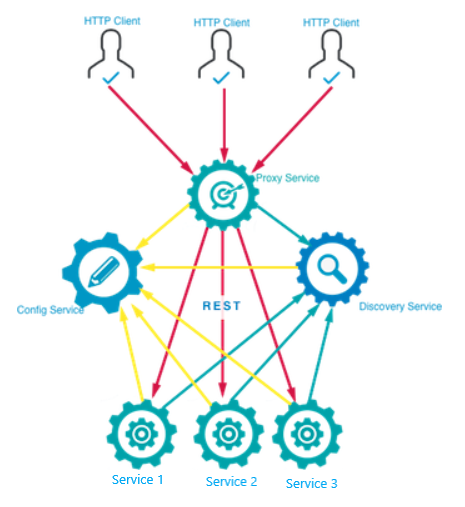
\includegraphics[width=0.5\linewidth]{images/tp01}
	\caption{Architecture Spring cloud et Netflix  par des microservices}
	\label{fig:tp01}
\end{figure}


\subsection{Création des Microservices}
\subsubsection{Microservice  Service 1}
Nous commençons par la création du service principal: Service 1.

\begin{figure}[H]
	\centering
	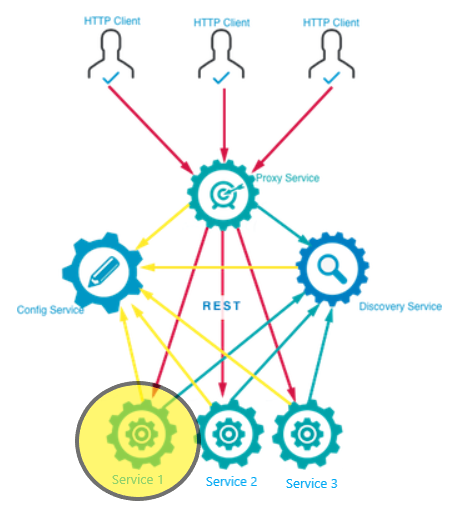
\includegraphics[width=0.5\linewidth]{images/tp02}
	\caption{Microservice  Service 1}
	\label{fig:tp02}
\end{figure}


Chaque microservice aura la forme d'un projet Spring. Pour créer rapidement et facilement un projet Spring avec toutes les dépendances nécessaires, Spring Boot fournit Spring Initialisé, il faut accéder  au site \underline{\textbf{start.spring.io}}, et créer un projet avec les caractéristiques suivantes:

\begin{enumerate}
       	\item  Projet Maven avec Java et Spring Boot version 2.0.1
		\item  Group: tn.insat.tpmicro
		\item  Artifact: User-service
		\item  Dépendances:
		
		\begin{itemize}
		  \item Web
		  \item Rest Repositories
		  \item JPA : Java Persistence API
		 \item Mysql : base de données pour le stockage
		 \item Actuator : pour le montoring et la gestion de l'application
		 \item  Eureka Discovery : pour l'intégration avec le Discovery Service
		 \item  Config Client : pour l'intégration avec le Config Service
		\end{itemize}
		



Suivre ensuite les étapes suivantes pour créer le microservice UserService:

\begin{itemize}
\item Ouvrir le projet téléchargé avec votre éditeur. 

\item Sous le répertoire src/main/java et dans le package com.example.entitis, créer la classe User  \textbf{(voir annexe A.1) }.
\end{itemize}



\item Cette classe est annotée avec JPA, pour stocker ensuite les objets user dans la base de données mysql grâce à Spring Data. Pour cela, créer l'interface UserRepository dans le même package  \textbf{(voir annexe A.2) }. 




\item Pour insérer les objets dans la base, nous utiliserons l'objet Stream. Pour cela, nous allons créer la classe DummyDataCLR \textbf{(voir annexe A.3)}.



\item Nous remarquons ici que le UserRepository sera instancié automatiquement grâce au mécanisme d'injection de dépendances, utilisé par Spring.

Lancer la classe principale. Une base de données MySql sera créée et le CommandLineRunner se chargera de lui injecter les données.


\begin{att}
	Prenez soin d'utiliser JDK 8!
\end{att}


\item Pour exécuter votre application:

  * Créer une configuration mvn package par l'éditeur  
    
        
    
  * Lancer ensuite la configuration Spring Boot UserServiceApplication  
  
    
\end{enumerate}
    
    
     
    
    
        
    \subsubsection{Microservice ConfigService}    
    Dans une architecture microservices, plusieurs services s'exécutent en même temps, sur des processus différents, avec chacun sa propre configuration et ses propres paramètres. Spring Cloud Config fournit un support côté serveur et côté client pour externaliser les configurations dans un système distribué. Grâce au service de configuration, il est possible d'avoir un endroit centralisé pour gérer les propriétés de chacun de ces services
    
    \begin{figure}[H]
    	\centering
    	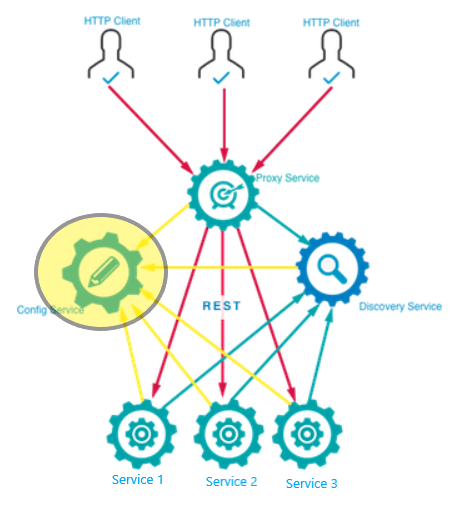
\includegraphics[width=0.5\linewidth]{images/tp03}
    	\caption{Microservice ConfigService}
    	\label{fig:tp03}
    \end{figure}
    
    Pour cela:      
    \begin{enumerate}
    	
    	\item  Commencer par créer un service ConfigService dans Spring Initializr, avec les dépendances appropriées, comme indiqué sur la figure suivante:
    	
    	
    	
    	\item  Ouvrir le projet dans une autre instance d'IntelliJ IDEA.
    	
    	\item  Pour exposer un service de configuration, utiliser l'annotation\\
    	\textbf{@EnableConfigServer} pour la classe \textbf{ConfigServiceApplication}, \textbf{(Voir annexe B.1)}  
    	\item  Pour paramétrer ce service de configuration, ajouter dans son fichier application.properties les valeurs suivantes:
    	
\begin{lstlisting}
server.port=8888
spring.cloud.config.server.git.uri=file:./src/main/resources/myConfig
\end{lstlisting}
    	
    	Ceci indique que le service de configuration sera lancé sur le port 8888 et que le répertoire contenant les fichiers de configuration se trouve dans le répertoire src/main/resources/myConfig. Il suffit maintenant de créer ce répertoire.
    	
    	
    	\item  Créer le répertoire myConfig à l'arborescence src/main/resources
    	
    	\item  Créer dans ce répertoire le fichier application.properties dans lequel vous insérez l'instruction suivante:
    	\begin{lstlisting}
global=xxxxx
    	\end{lstlisting}
    	
    	Ce fichier sera partagé entre tous les microservices utilisant ce service de configuration.
    	
    	\item Le répertoire de configuration doit être un répertoire git. Pour cela:
    	
    	\begin{itemize}
    		\item Ouvrir le terminal avec IntelliJ et naviguer vers ce répertoire.
    		\item  Initialiser votre répertoire:\textbf{ git init}
    		\item  Créer une entrée racine dans le repository: \textbf{git add .}
    		\item  Faire un commit: \textbf{git commit -m "add ."}
    	\end{itemize}
    	
    	Revenir vers le projet ProductService et ajouter dans le fichier de configuration application.properties:
\begin{lstlisting}
spring.application.name = product-service
spring.cloud.config.uri = http://localhost:8888
\end{lstlisting}
    	
    	Redémarrer vos services. Pour consulter le service de configuration, aller à {\color{red} http://localhost:8888/product-service/master}. 
    	
    	Vous verrez le fichier JSON  \textbf{(Voir annexe B.2)}
    
    	Comme le fichier application.properties contient toutes les propriétés partagées des différents microservices, nous aurons besoins d'autres fichiers pour les propriétés spécifiques à un microservice. Pour cela:
    	
    	\item Créer dans le répertoire myConfig un fichier product-service.properties pour le service ProductService.
    	
    	\item  Ajouter les propriétés de votre service, à savoir, par exemple:
    	
\begin{lstlisting}
me=Djamel.Zerroukki@jimmi.fr
\end{lstlisting} 
    	
    	Relancer le microservice de configuration. En consultant l'url {\color{red}http://localhost:8888/product-service/master}, nous remarquons l'ajout de la nouvelle propriété.\textbf{(Voir annexe B.3)}
    	 
    	Nous allons maintenant définir un appel REST à cette propriété. Pour cela:
    	
    	\item Créer la classe ProductRestService dans le projet product-service.\textbf{(Voir annexe B.4)}
    	
  
    	
    	
    	\item Redémarrer l'instance  du service, puis appeler dans votre navigateur le service en tapant: {\color{red} http://localhost:8080/messages}. 
    	
    	
    	
    \end{enumerate}
    
    
    
    
    
    
    \subsubsection{Microservice DiscoveryService}
Pour éviter un couplage fort entre microservices, il est fortement recommandé d'utiliser un service de découverte qui permet d'enregistrer les propriétés des différents services et d'éviter ainsi d'avoir à appeler un service directement. Au lieu de cela, le service de découverte fournira dynamiquement les informations nécessaires, ce qui permet d'assurer l'élasticité et la dynamicité propres à une architecture microservices.
\begin{figure}[H]
	\centering
	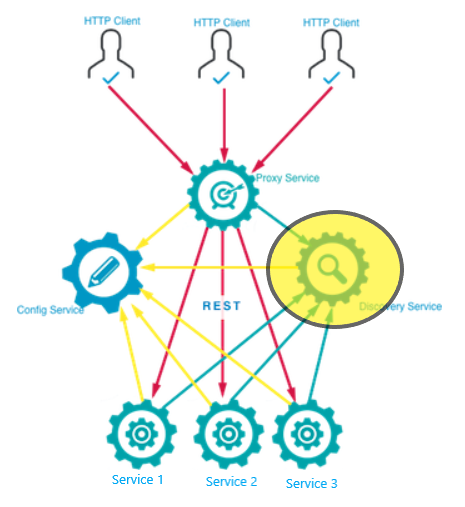
\includegraphics[width=0.5\linewidth]{images/tp04}
	\caption{Microservice DiscoveryService}
	\label{fig:tp04}
\end{figure}
    
    Pour réaliser cela, Netflix offre le service \textbf{Eureka Service Registration and Discovery}, que nous allons utiliser dans notre application.
    
    
    \begin{enumerate}
\item Revenir à Spring Initializr et créer un nouveau projet Spring Boot intitulé discovery-service avec les dépendances Eureka Server et Config Client.
\item Lancer le projet avec votre éditeur.
\item Dans la classe DiscoveryServiceApplication, ajouter l'annotation \textbf{@EnableEurekaServer}. \textbf{(Voir annexe C.1)} 

\item  Ajouter les propriétés suivantes dans son fichier application.properties.

\begin{lstlisting}
spring.application.name=discovery-service
spring.cloud.config.uri=http://localhost:8888
\end{lstlisting}

\item Dans le projet config-service, créer un fichier discovery-service.properties sous le répertoire myConfig.

\item Ajouter les propriétés suivantes pour (1) définir le port par défaut du service de découverte et (2) empêcher un auto-enregistrement du service Eureka.

\begin{lstlisting}
server.port = 8761
eureka.client.fetch-registry = false
eureka.client.register-with-eureka = false
\end{lstlisting}

Pour consulter le service Eureka, aller à {\color{red}  http://localhost:8761}, l'interface suivante s'affiche:



    \end{enumerate}
    
    
    \subsubsection{Microservice ProxyService}
    L'architecture microservice, en fournissant un ensemble de services indépendants et faiblement couplés, se trouve confrontée au challenge de fournir une interface unifiée pour les consommateurs, de manière à ce qu'ils ne voient pas la décomposition à faible granularité de vos services. C'est pour cela que l'utilisation d'un service proxy, responsable du routage des requêtes et de la répartition de charge, est important.
    
    \begin{figure}[H]
    	\centering
    	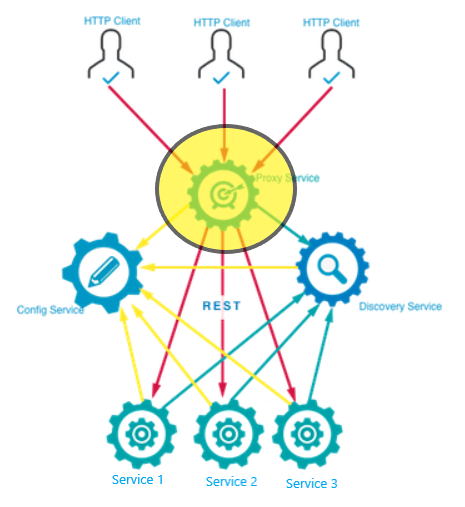
\includegraphics[width=0.5\linewidth]{images/tp05}
    	\caption{Microservice ProxyService}
    	\label{fig:tp05}
    \end{figure}
    
    Netflix offre le service \textbf{Zuul} pour réaliser cela. Pour créer votre microservice Proxy:
    \begin{enumerate}
\item    Aller à Spring Initializr.
\item     Créer le projet proxy-service avec les dépendances suivantes: \textbf{(Zuul, Web, HATEOAS, Actuator, Config Client et Eureka Discovery )}.
\item     Ouvrir le service avec votre  IDEA.
\item     Ajouter à la classe ProxyServiceApplication l'annotation \textbf{@EnableZuulProxy} \textbf{(Voir annexe C.1)} , ainsi que \textbf{@EnableDiscoveryClient} pour que le proxy soit également enregistré dans le service ce découverte.\textbf{(Voir annexe D.1)}
\item     Ajouter les propriétés spring.application.name et spring.cloud.config.uri dans le fichier application.properties du service proxy.
\item     Créer le fichier proxy-service.properties dans le répertoire myConfig du service de configuration, dans lequel vous allez fixer le port du service proxy à 9999.
 \end{enumerate}


En lançant le service Proxy, vous remarquerez qu'il est rajouté dans Eureka.
    
    
    
      \subsection{Consulter les services via le proxy }
    le diagramme de séquence de la figure \ref{fig:secance}   exprime  la  consultation des services via le proxy 
    \begin{enumerate}
    	
    	\item Un client HTTP envoie la requête HTTP vers le proxy qui contient le nom de micro service.  
    	
  
    	
    		\item  Le service proxy connaît le nom de micro service, il va demander au service de registration l'emplacement de la machine où se trouve ce micro-service. 
    
    	\item Le service de registration  va retourner l'adresse IP et le port s'il a une instance ou  une liste s'il a  plusieurs instances.
    	
    	\item  Le service proxy va choir une instance et  va envoyer la requête.  
    	
    	\item  Le service demandé va faire le traitement ensuite envoie le résultat vers le proxy qui va le transmettre au client. 
    \end{enumerate}
    
    
    \begin{figure}[H]
    	\centering
    	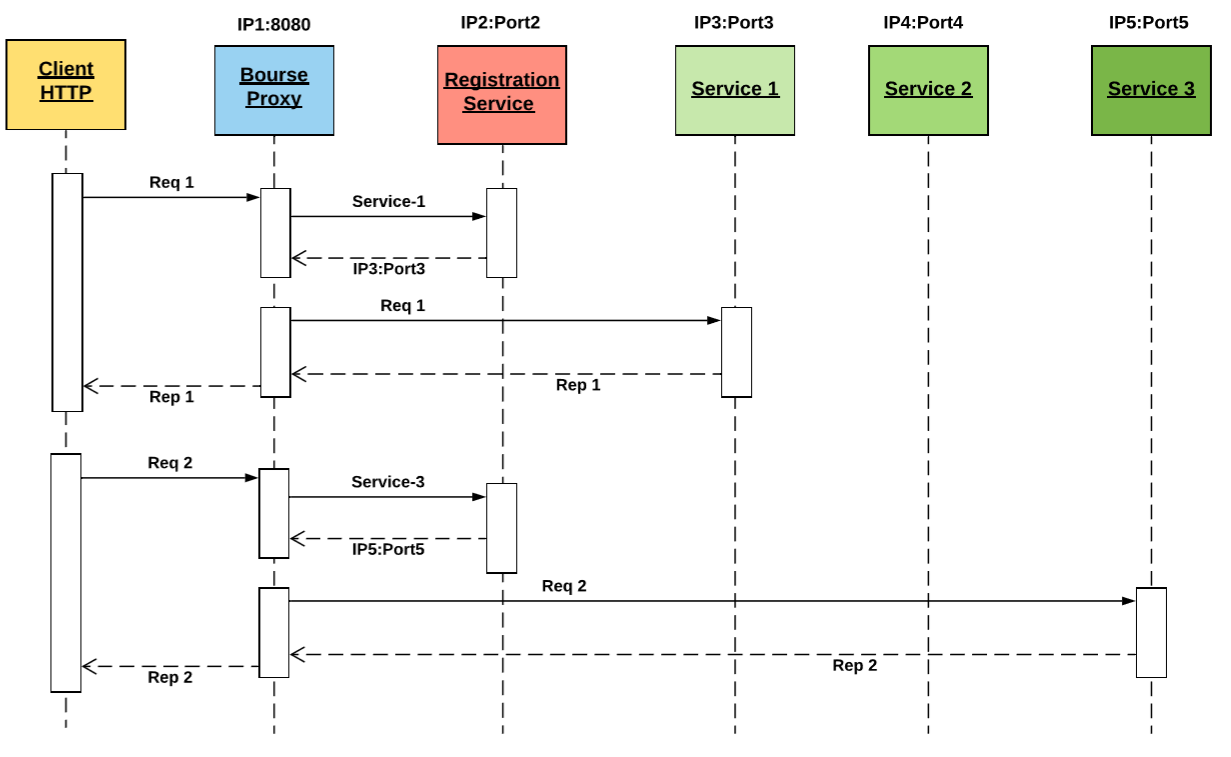
\includegraphics[width=1\linewidth]{images/secance}
    	\caption{Diagramme séquence représenté comment  Consulter les services via le proxy}
    	\label{fig:secance}
    \end{figure}
    
    
    
    
    
    \section{Description de l'architecture de notre système}
    
   \comment{ 
    
   \begin{figure}
    	\centering
    	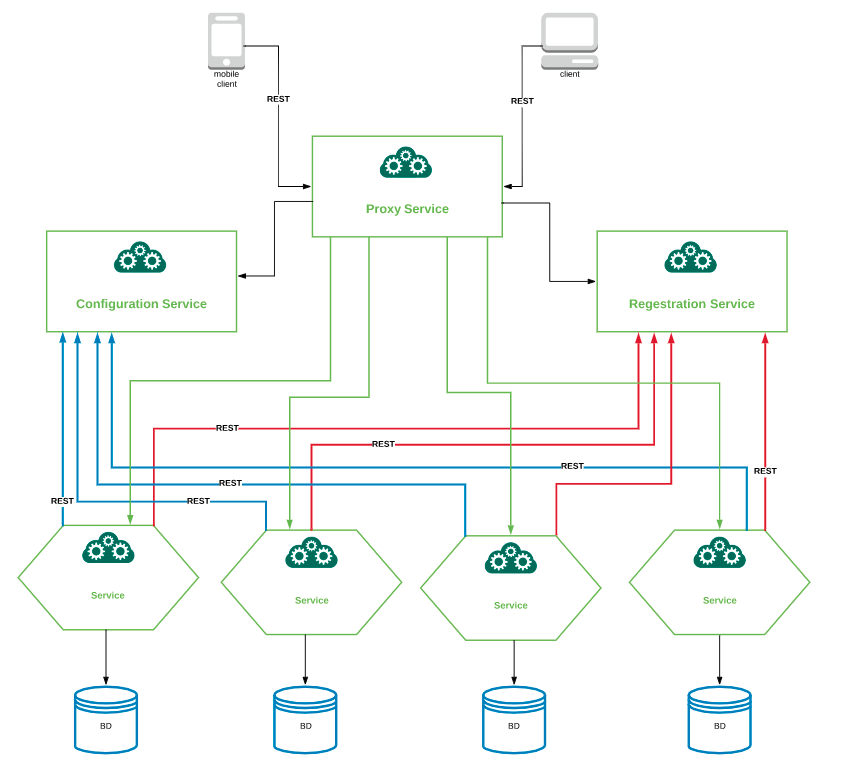
\includegraphics[width=1\linewidth]{images/arch}
    	\caption{ }
    	\label{fig:arch}
    \end{figure}

\begin{figure}[H]
	\centering
	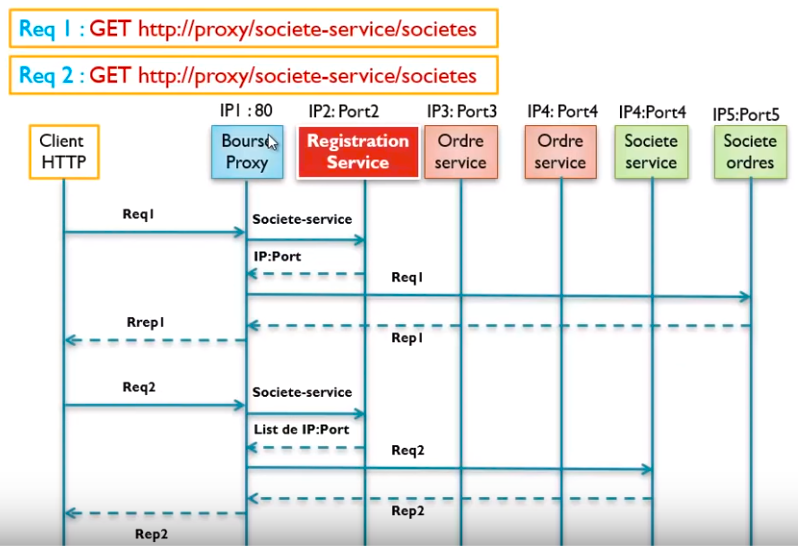
\includegraphics[width=1\linewidth]{images/mcservc}
	\caption{}
	\label{fig:mcservc}
\end{figure}

}
Nous avons instanciés le workflow dans plusieurs dimensions des cas (voir le paragraphe 1.3.4.2).         
 
 
    Nous avons développé  trois services pour l'orchestration des Micro-Service a  savoir service proxy, service  configuration et service  registration comme le montre  la figure \ref{fig:cloudms}.
    
De plus, nous avons développé un master service qui permettre d'instancier le workflow pour diverses organisations.  Autrement dit, le fournisseur de services offre ses services via le master service.
 \begin{figure}[H]
 	\centering
 	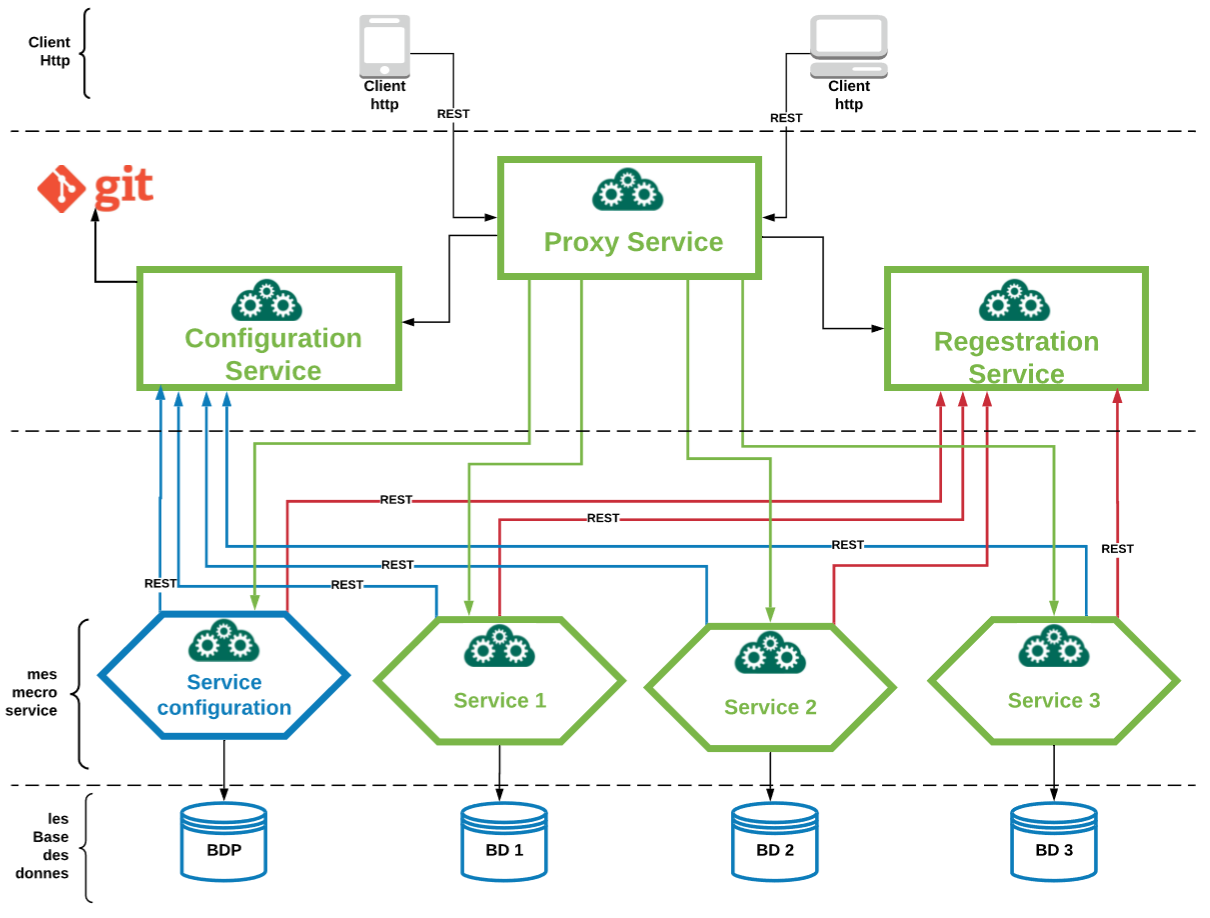
\includegraphics[width=1\linewidth]{images/cloudMS}
 	\caption{Notre architecture de système sur l'environnement Spring cloud et micro-service}
 	\label{fig:cloudms}
 \end{figure}
 
     Suite à la demande de la \ac{cnr} nous avons instanciés notre workflow pour cette organisation et nous avons amélioré notre application suivent  leur  cahier des charges  (Voir \textbf{Annexe C} qui représente  L'organigramme de la CNR).  
     
          
\subsection{Obstacles}
Nous avons essayé d'ouvrir un compte auprès des fournisseurs de services cloud cités dans la section 1.2.5 , pour déployer les services que nous avons développés, malheureusement sont tous payants.
 
  
  
 \section{Présentation de système }

 

 \subsection{Interface de l'administrateur }
  \subsubsection{Authentification}
Cette interface est la fenêtre de bienvenue.
Pour améliorer la sécurité du système, il est nécessaire de vérifier la disponibilité du compte d'utilisateur et le mot de passe est correct à ce niveau.
 \begin{figure}[H]
 	\centering
 	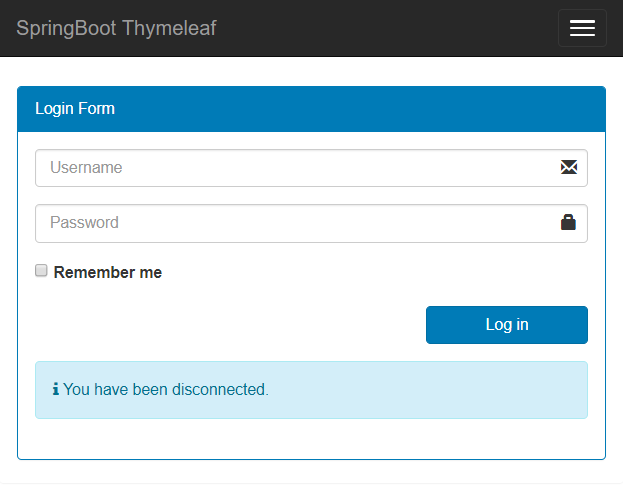
\includegraphics[width=1\linewidth,height=0.3\paperheight]{images/captures/capturesadmin/login}
 	\caption{Authentification au système }
 	\label{fig:login}
 \end{figure}
  
  
  
  
 \subsubsection{Création d'un circuit workflow}
L'administrateur peut créer un circuit de n'importe quel dossier via une interface graphique simple et utile.
\begin{exmp}
 Création d'un workflow pour un service de la \ac{cnr} comme illustré à la figure \ref{fig:bpmn}. 
\end{exmp}
 
\begin{figure}[H]
	\centering
	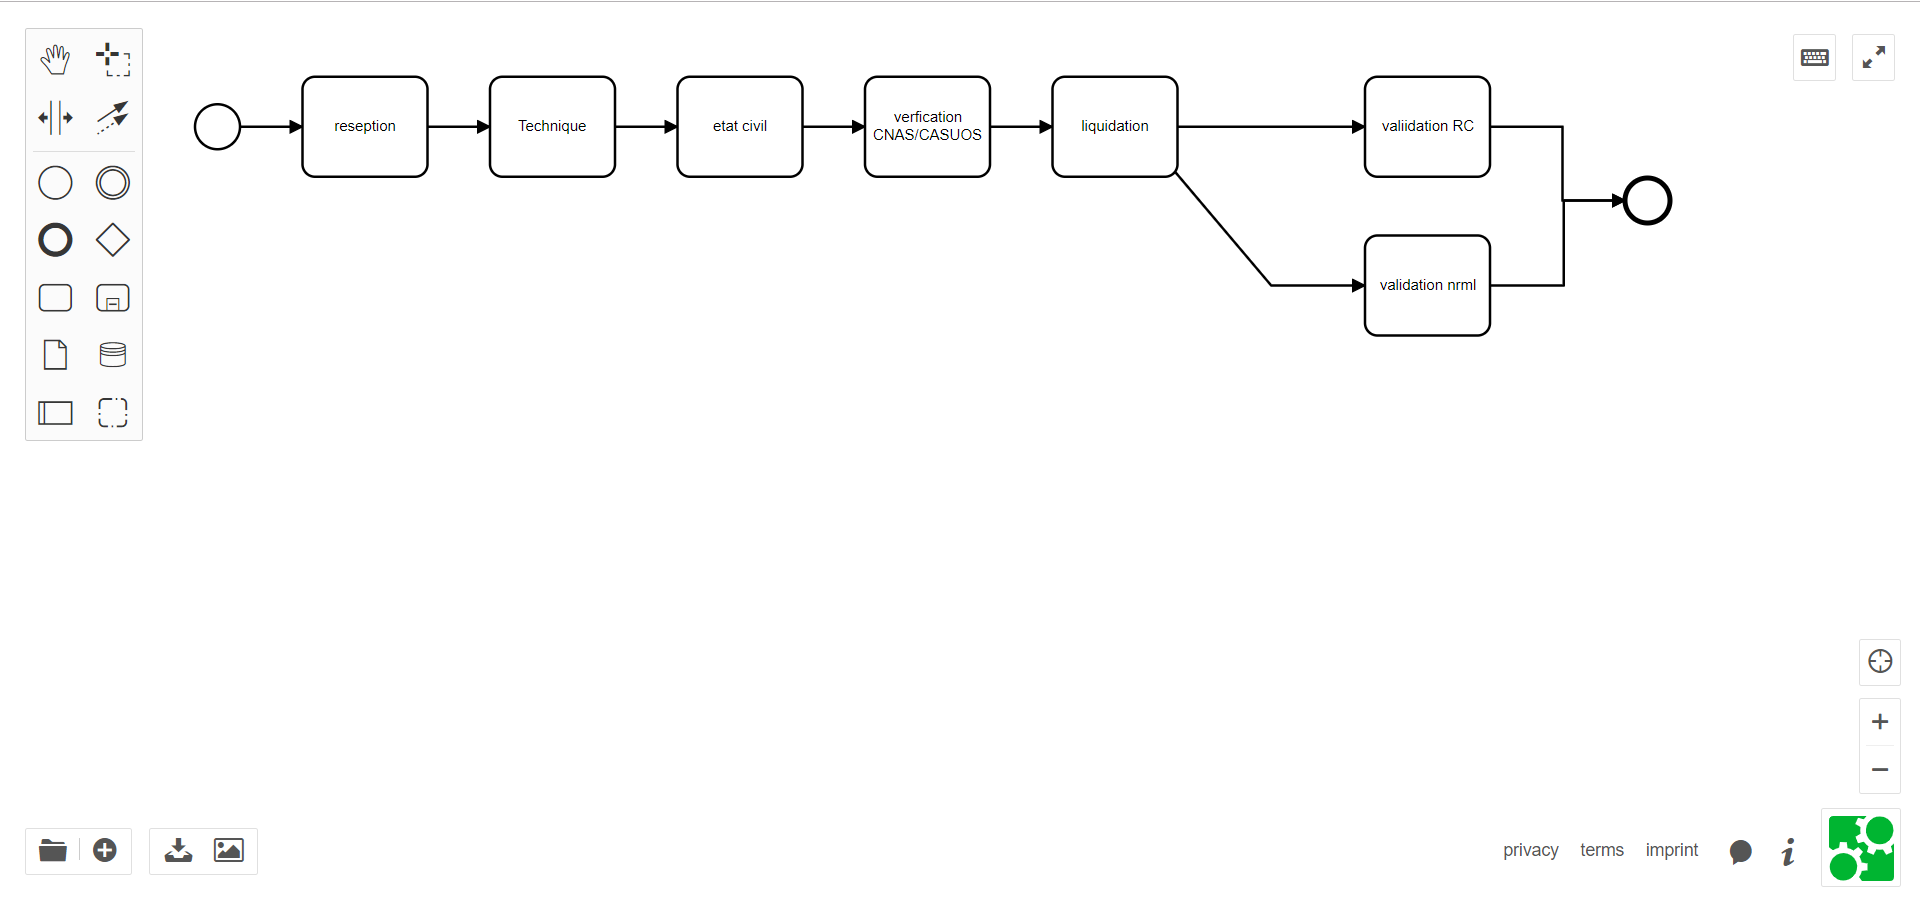
\includegraphics[width=1\linewidth,height=0.33\paperheight]{images/captures/capturesadmin/bpmn}
	\caption{Un workflow pour un service de la \ac{cnr}}
	\label{fig:bpmn}
\end{figure}
  
 
 
 
 \subsubsection{Gestion des Tâches }
L'administrateur peut gérer des tâches en modifiant des informations telles que le service et le temps de traitement. Il peut également afficher l'état des dossiers dans chaque tâche. 
\begin{figure}[H]
	\centering
	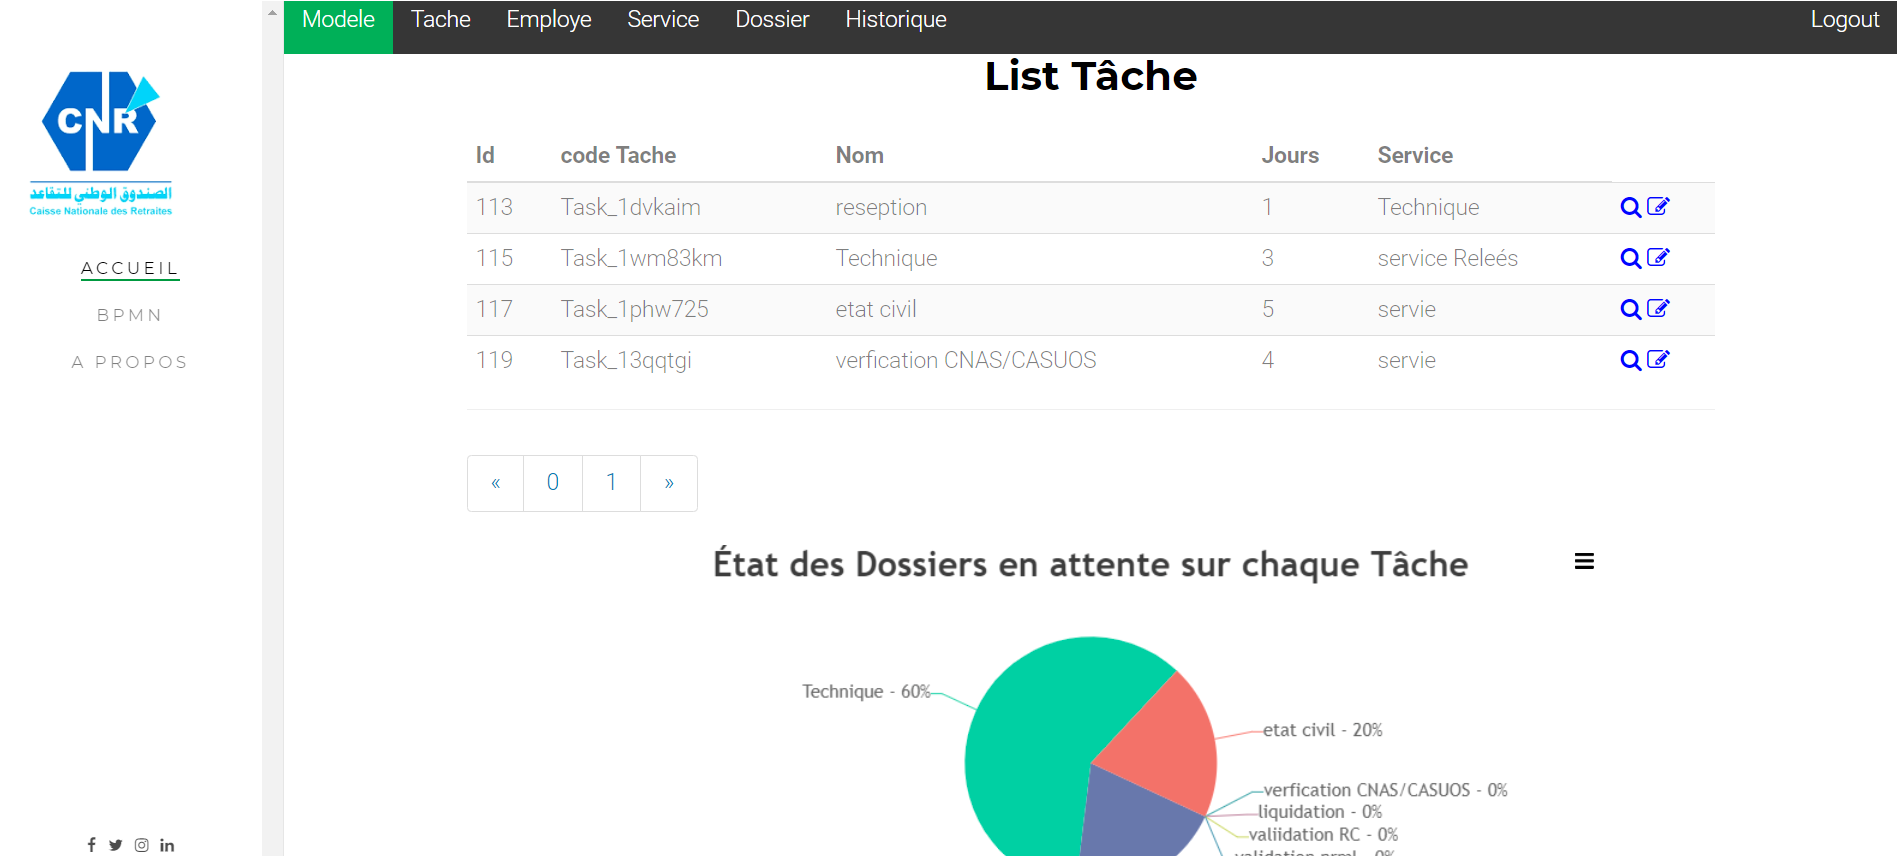
\includegraphics[width=1\linewidth,height=0.3\paperheight]{images/captures/capturesadmin/tache}
	\caption{Gestion des Tâches}
	\label{fig:tache}
\end{figure}

\subsubsection{ Consultation l'historique par Tâche }
L'administrateur peut consulter le résultat de la recherche par tâche et l'état actuel des dossiers. 
\begin{figure}[H]
	\centering
	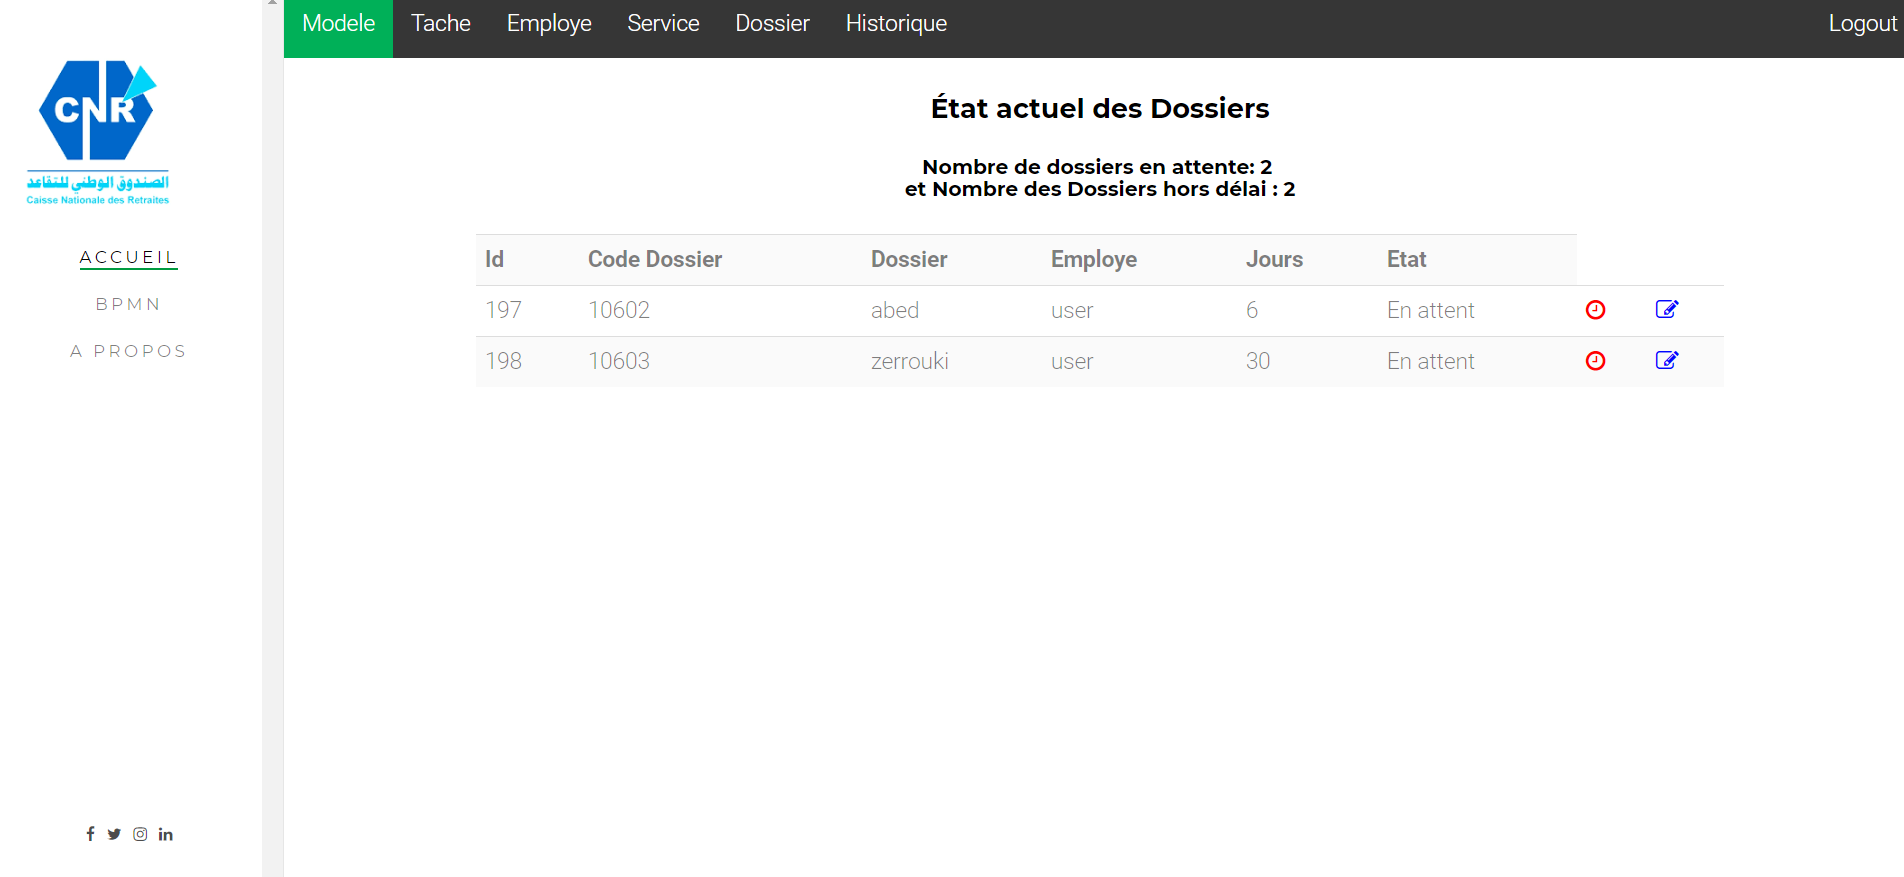
\includegraphics[width=1\linewidth]{images/captures/capturesadmin/HTache}
	\caption{Consultation Historique par Tâche}
	\label{fig:htache}
\end{figure}


\subsubsection{Gestion des  Sous-Directions et des Services }
L'administrateur peut gérer des sous-directions et des services en ajoutant et en modifiant leurs informations.
\begin{figure}[H]
	\centering
	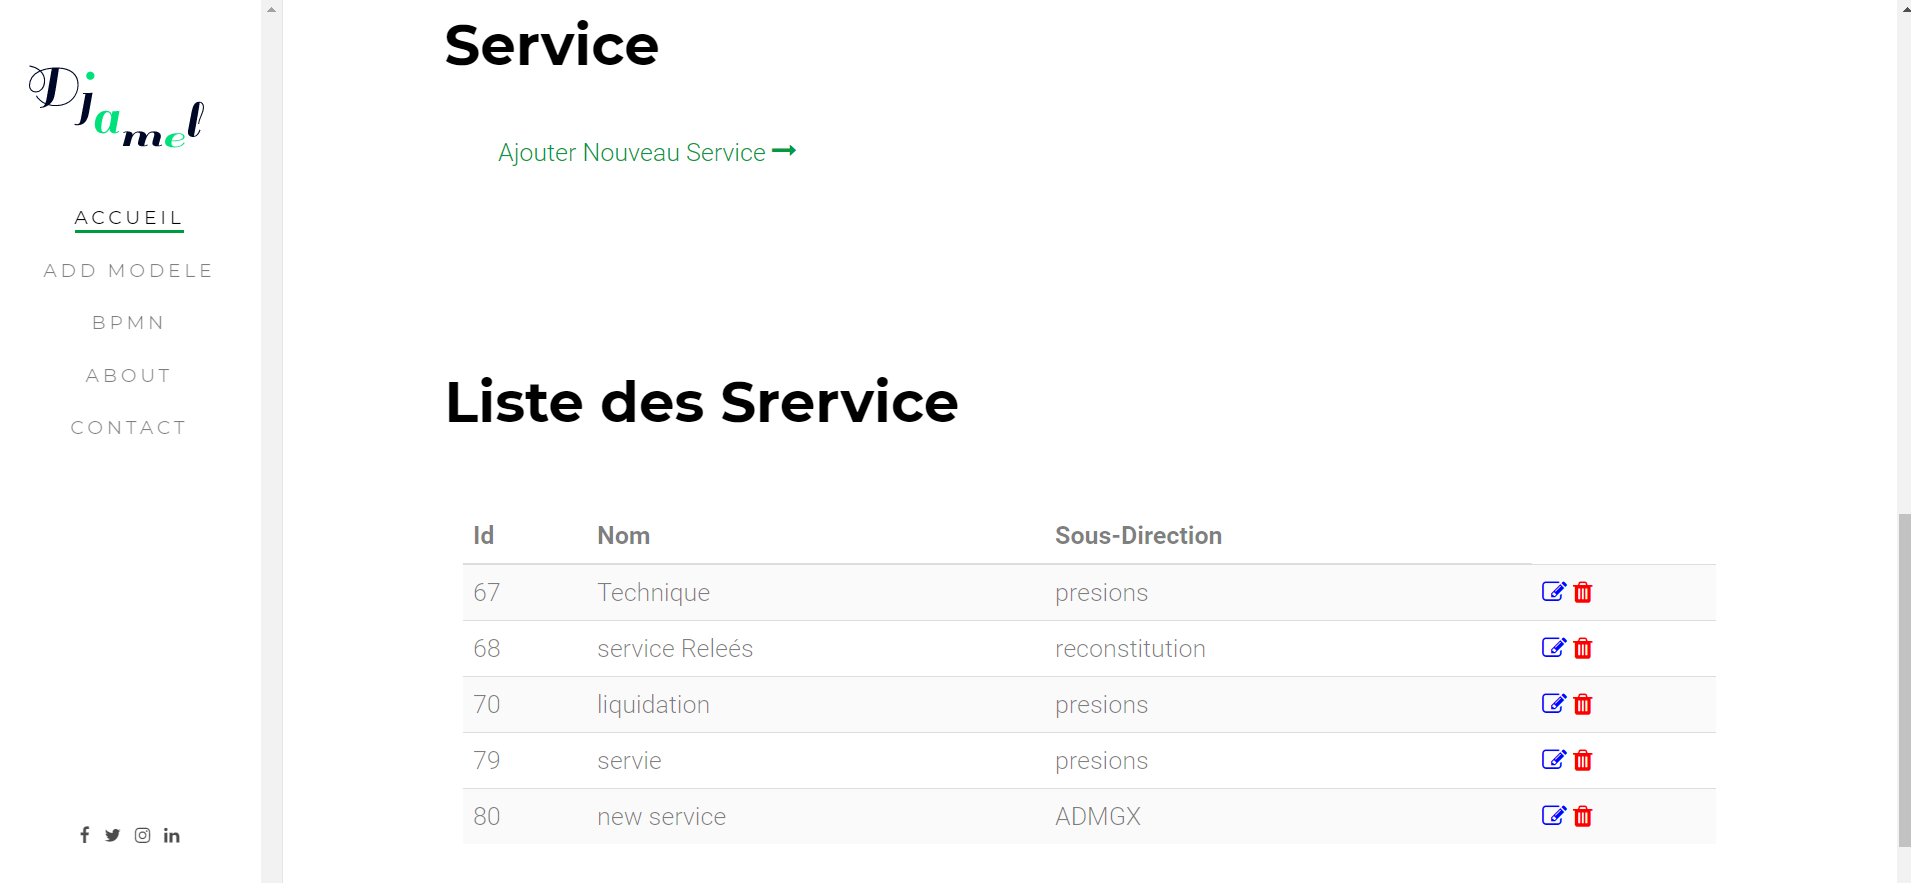
\includegraphics[width=1\linewidth,height=0.3\paperheight]{images/captures/capturesadmin/service}
	\caption{Gestion des  Sous-Directions et des Services}
	\label{fig:service}
\end{figure}


 
 \subsubsection{Gestion des  Utilisateurs}
 
 L'administrateur peut gérer les comptes d'utilisateurs en ajoutant, modifiant ou supprimant leurs informations.
\begin{figure}[H]
	\centering
	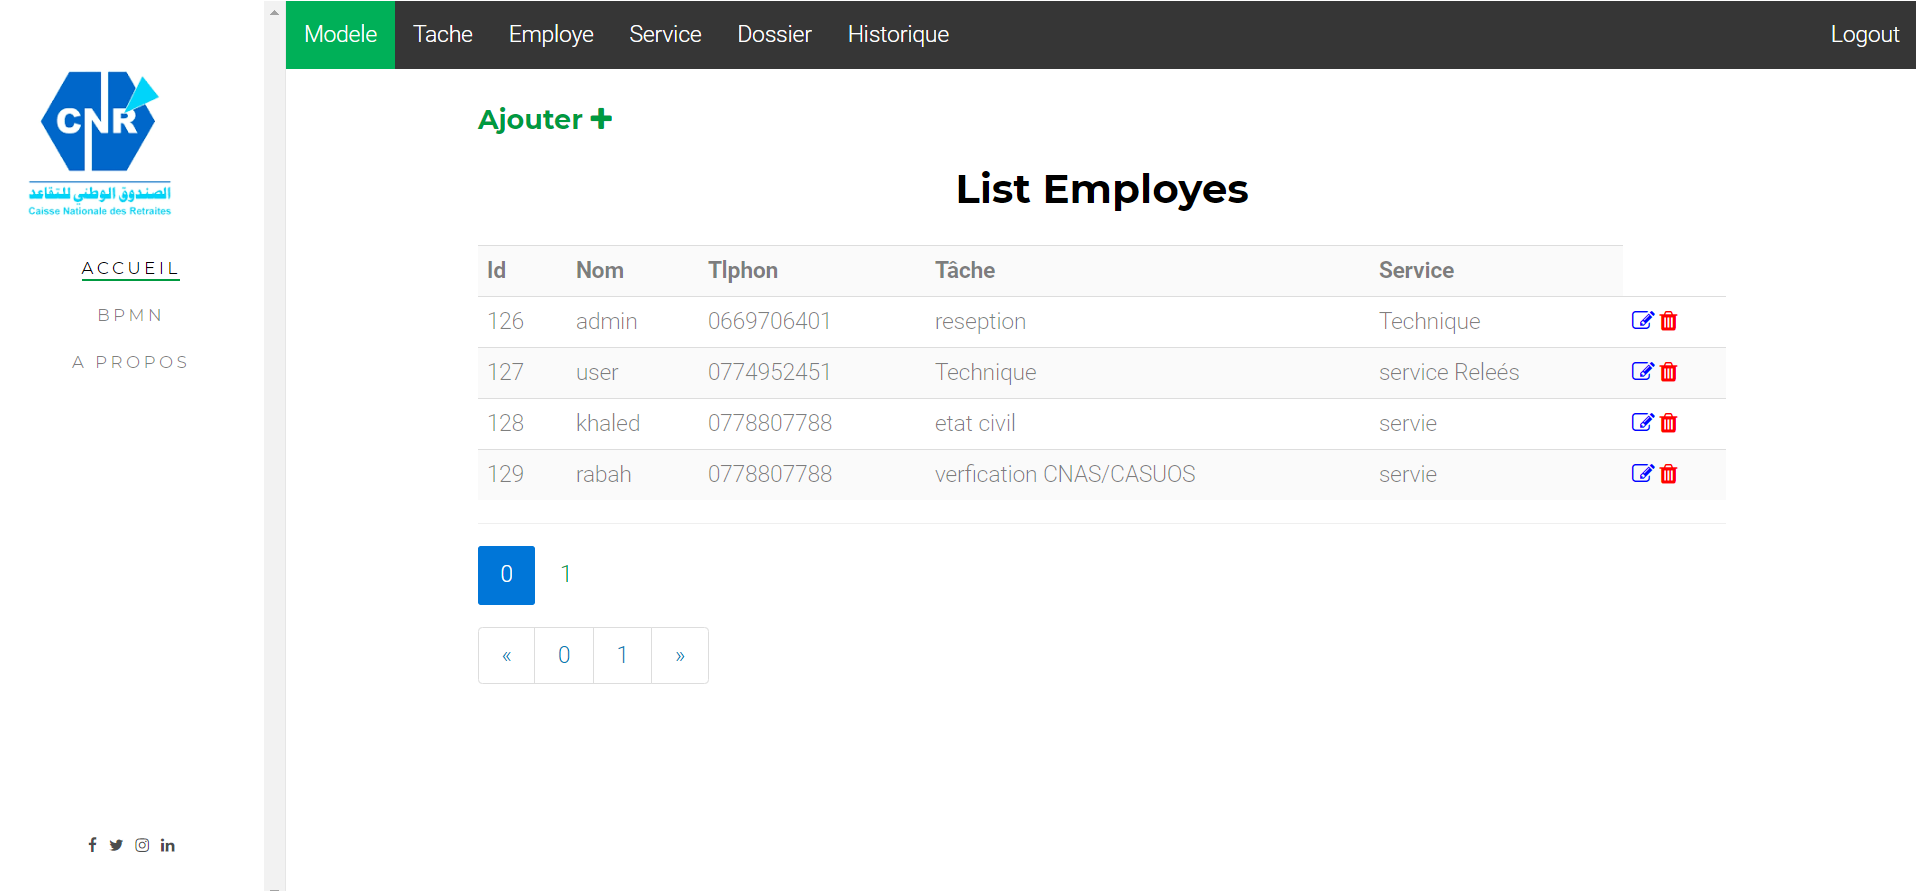
\includegraphics[width=1\linewidth,height=0.3\paperheight]{images/captures/capturesadmin/user}
	\caption{Gestion des  Utilisateurs}
	\label{fig:user}
\end{figure}




\subsubsection{Consultation des  Dossiers}
Cette page permet à l'administrateur de voir tous les dossiers en cours de traitement et son statut par la recherche.
\begin{figure}[H]
	\centering
	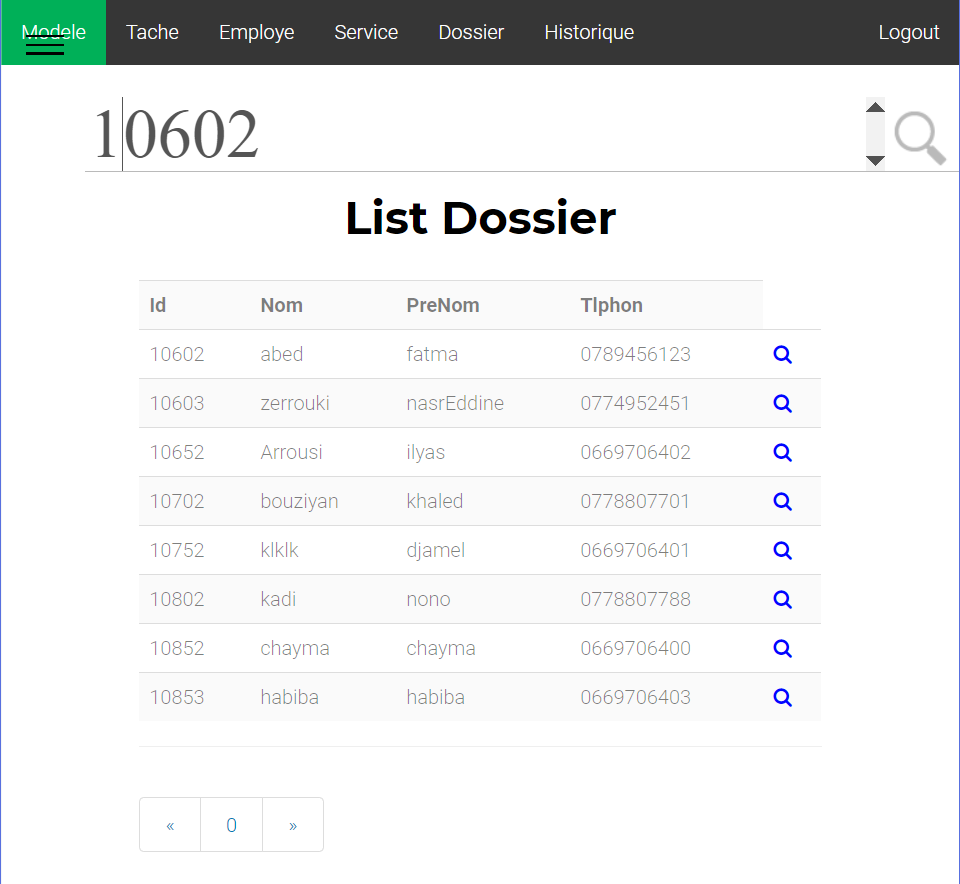
\includegraphics[width=1\linewidth]{images/captures/capturesadmin/dossier}
	\caption{Consultation des  Dossiers}
	\label{fig:dossier}
\end{figure}

\subsubsection{ Consultation l'historique par dossier }
Le résultat de la recherche est affiché par dossier comme suit:(figure \ref{fig:historique})
\begin{figure}[H]
	\centering
	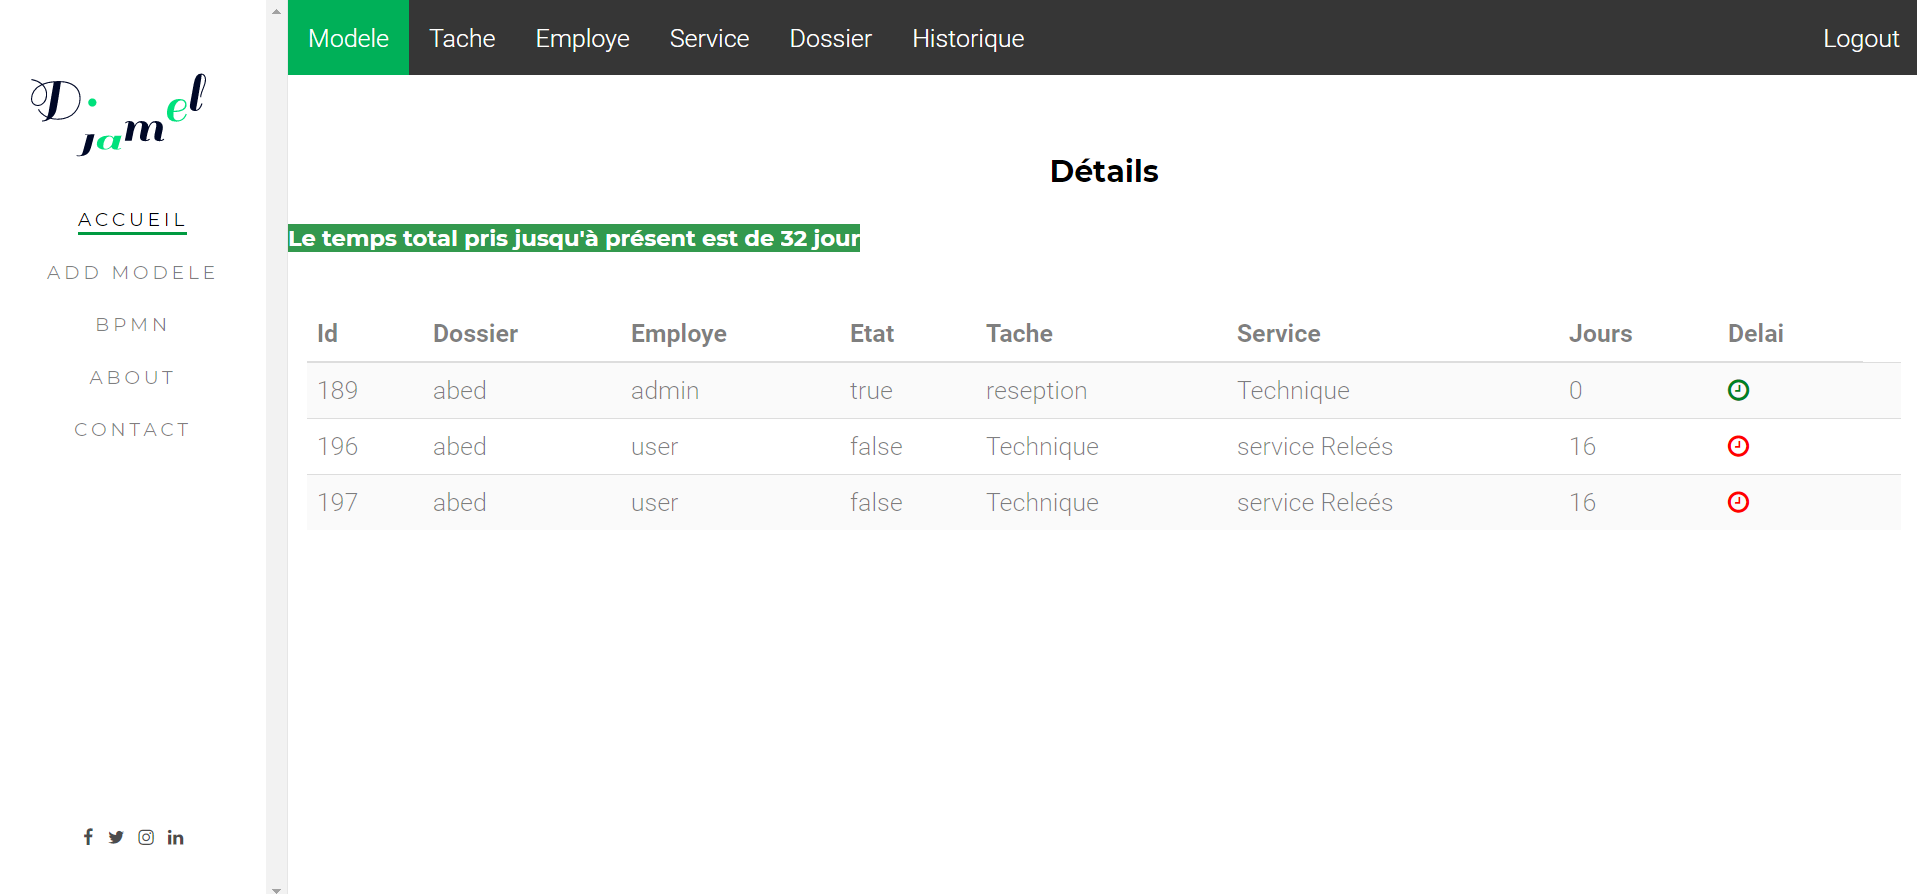
\includegraphics[width=1\linewidth,height=0.3\paperheight]{images/captures/capturesadmin/historique}
	\caption{Consultation Historique par dossier }
	\label{fig:historique}
\end{figure}

 

 \subsection{l'interfaces de l'Utilisateur }
\subsubsection{ Accueil  }
La page d'accueil pour des utilisateurs de système "les employés".
\begin{figure}[H]
	\centering
	
\includegraphics[width=1\linewidth,height=0.3\paperheight]{images/captures/capturesuser/home}
	\caption{Accule}
	\label{fig:home}
\end{figure} 




\subsubsection{Ajouter un dossier}

L'utilisateur de réception crée des dossiers sur cette interface en remplir toutes les informations et en vérifiant les champs.
\begin{figure}[H]
	\centering
	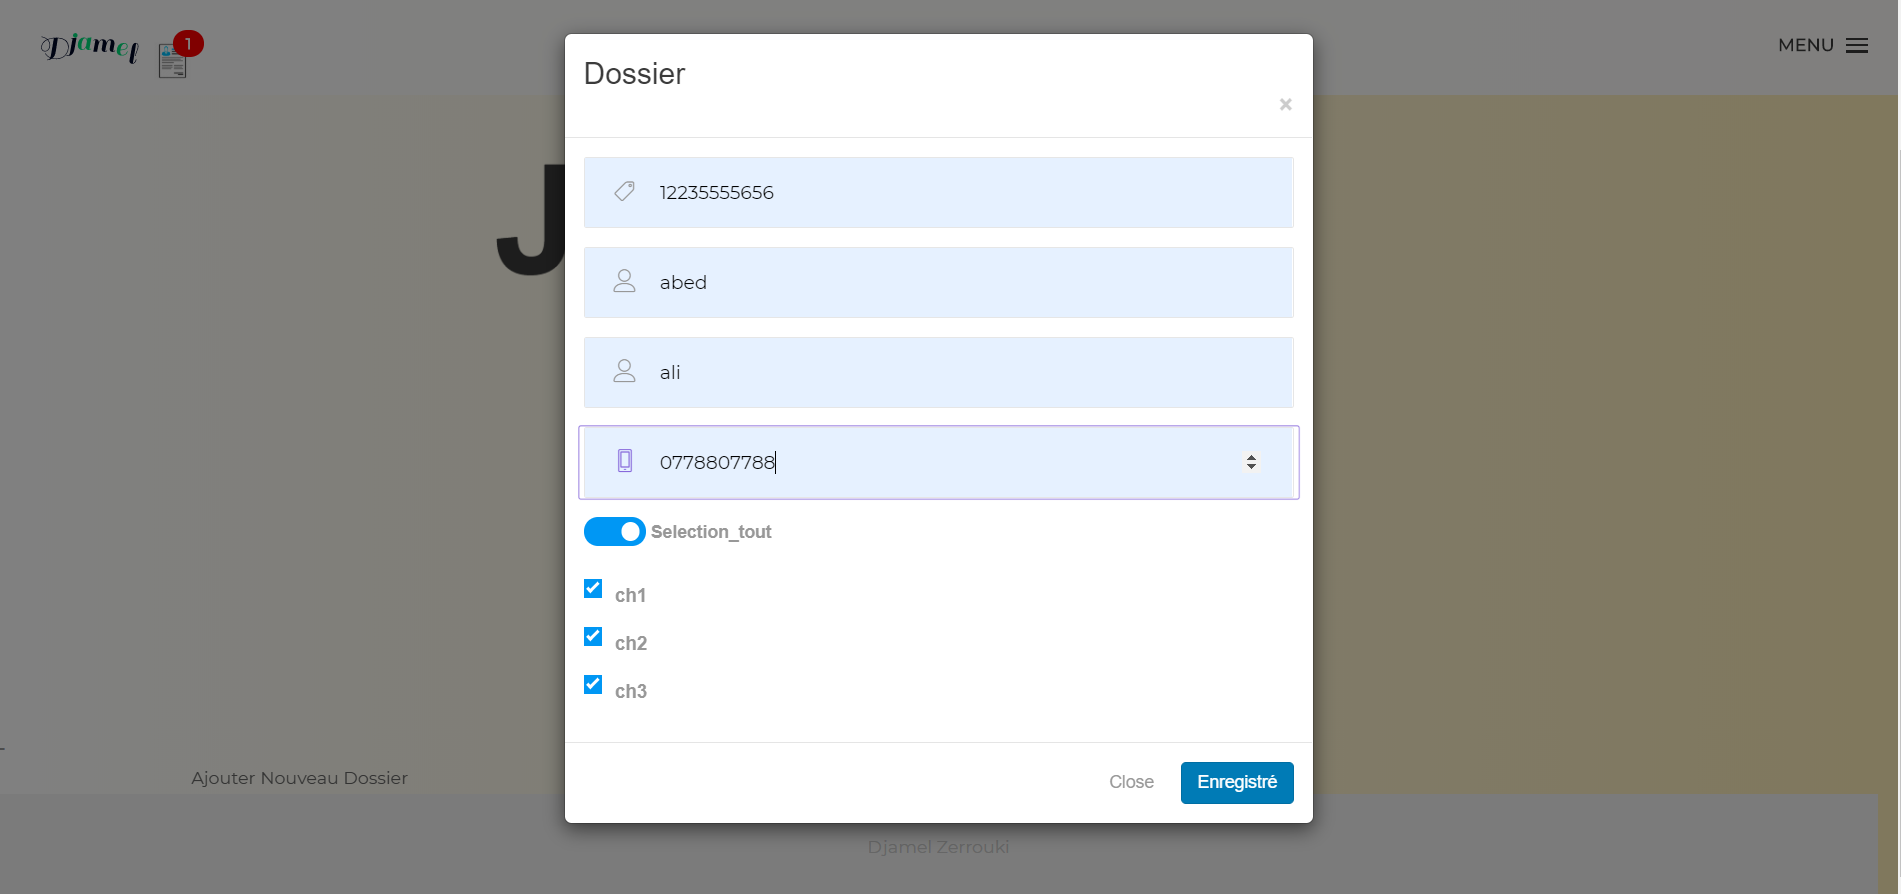
\includegraphics[width=1\linewidth]{images/captures/capturesuser/adddossier}
	\caption{Ajouter un dossier}
	\label{fig:adddossier}
\end{figure}



\subsubsection{ Liste des dossier }
Affichez et filtrez les dossiers de la manière suivante: "En attente", "Traitement en cours" ou "Tous les fichiers".
\begin{figure}[H]
	\centering
	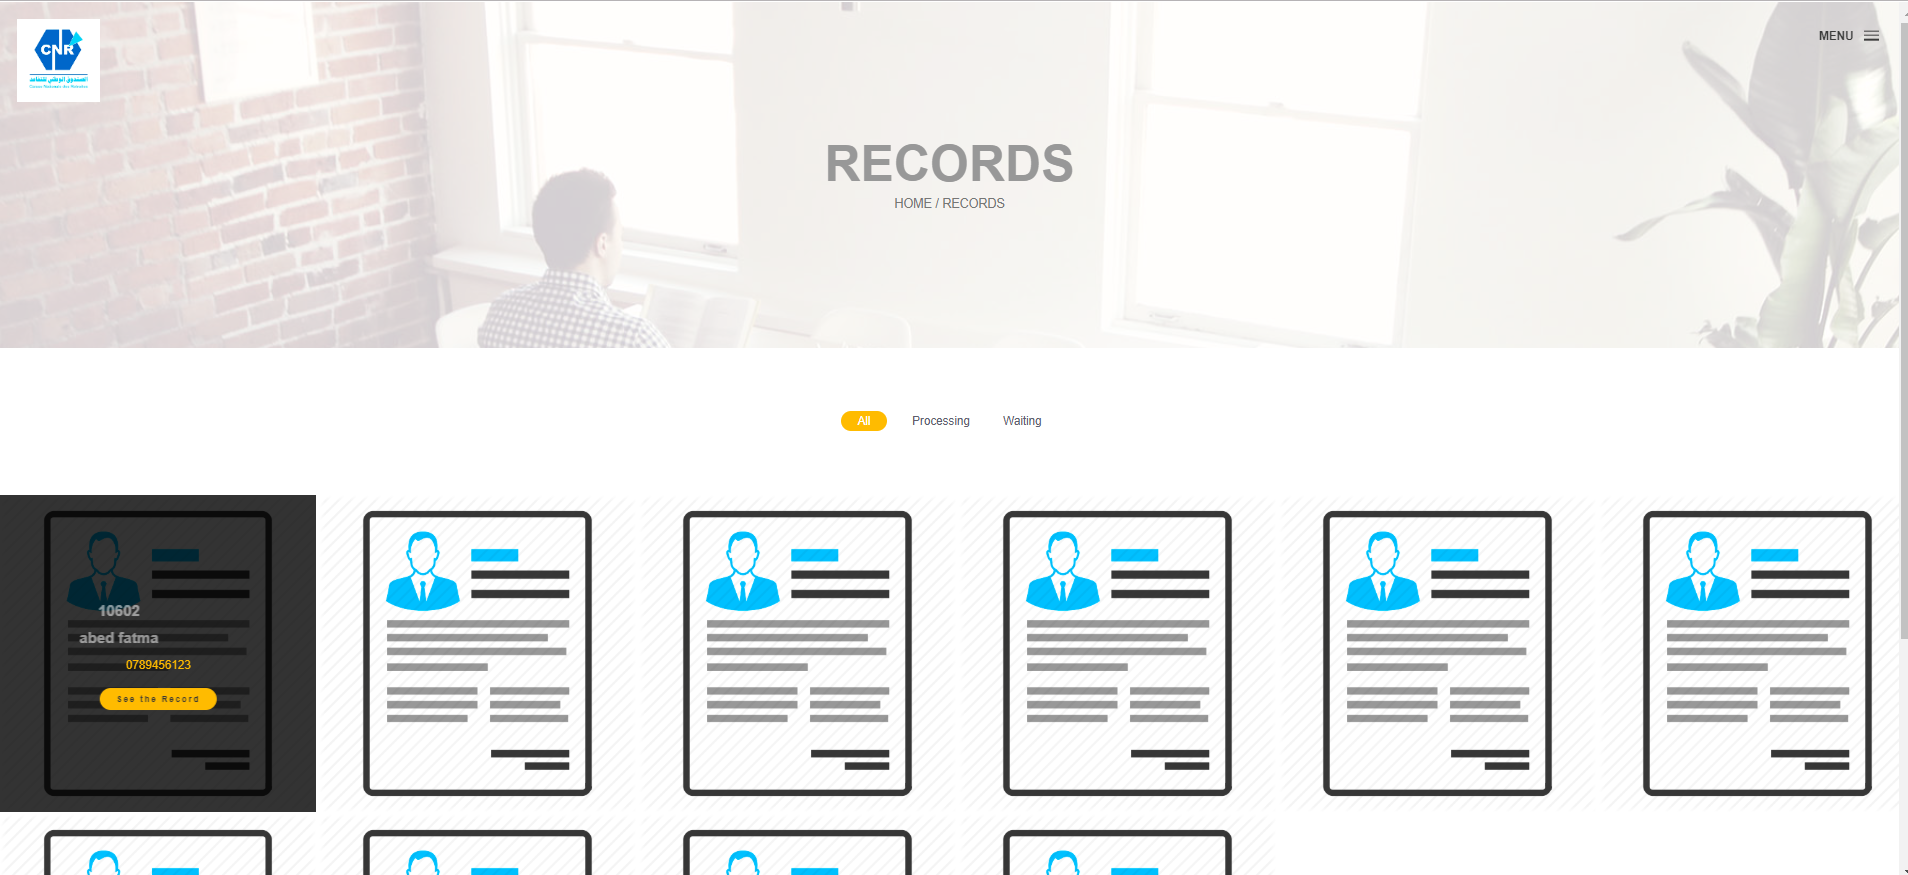
\includegraphics[width=1\linewidth]{images/captures/capturesuser/dossier}
	\caption{Liste des dossier}
	\label{fig:udossier}
\end{figure}


\subsubsection{ Gérer les  bordereaux }
L'utilisateur peut sélectionner liste des dossiers et créer un bordereau pour transformer et la gérer ("Accepter", "Refuses", "Imprimer").

 
\begin{figure}[H]
	\centering
	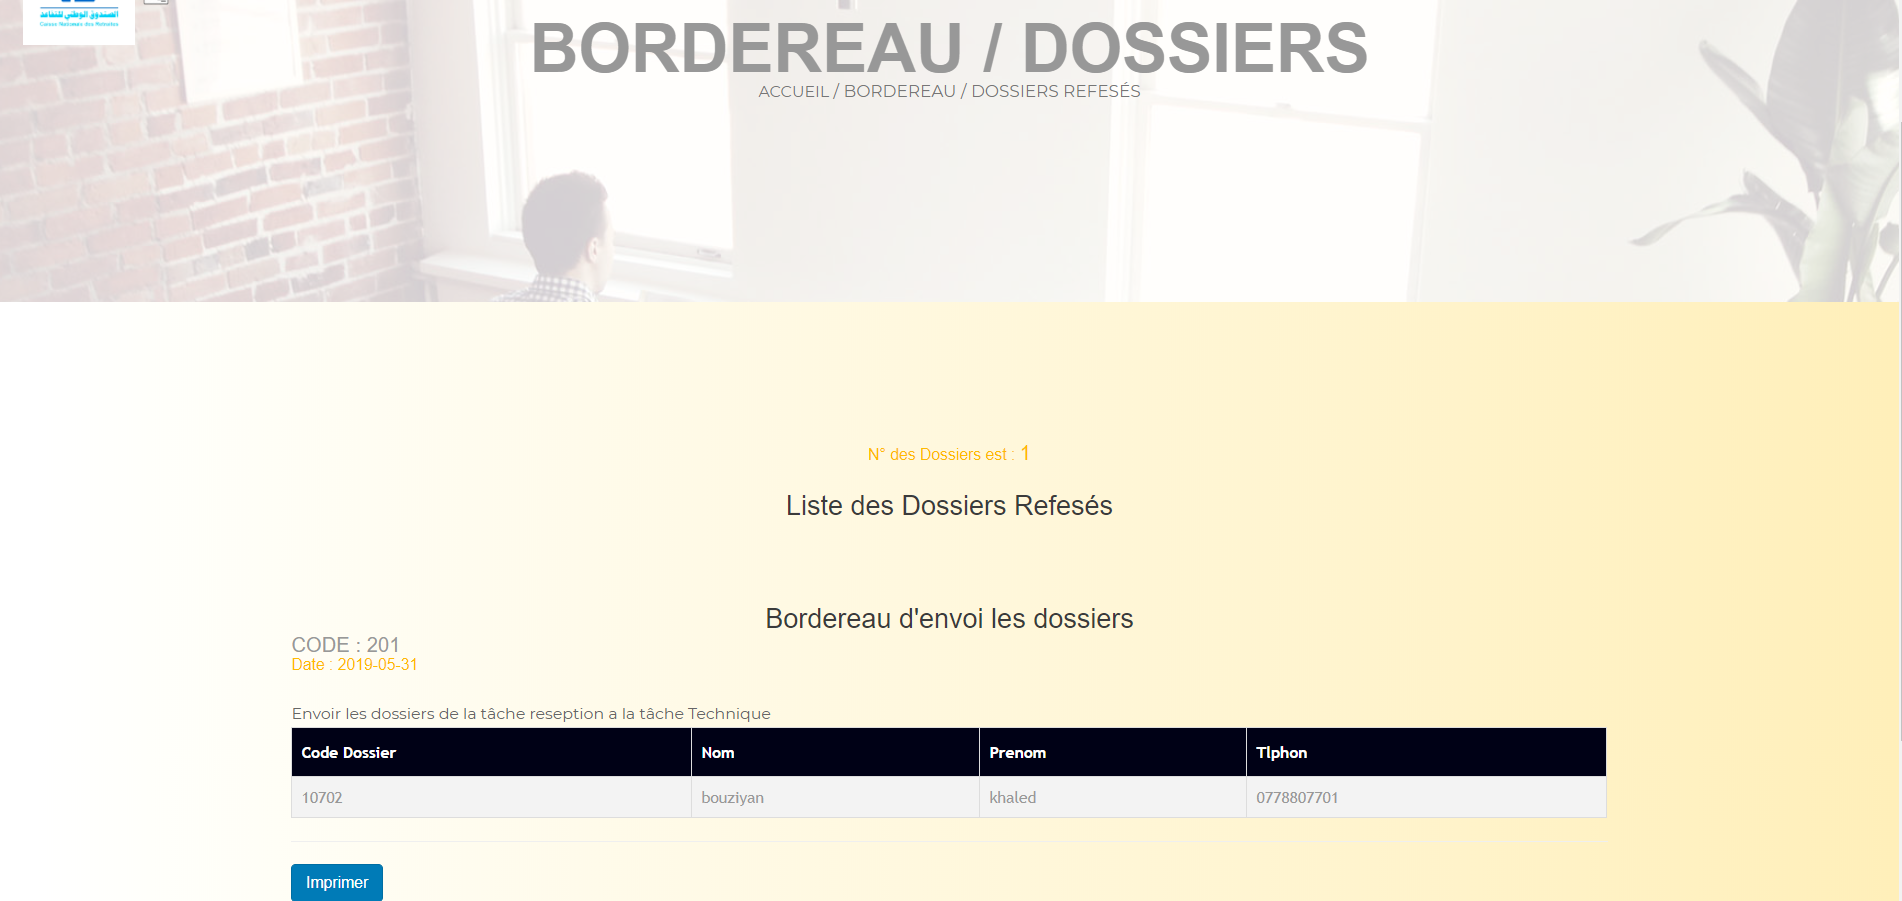
\includegraphics[width=1\linewidth]{images/captures/capturesuser/bord}
	\caption{Gérer les  bordereaux}
	\label{fig:bord}
\end{figure}



\section{Conclusion}

À travers ce chapitre, nous avons exposé l’architecture de la plateforme, les différents outils et technologies utilisées pour le développement d'un service cloud. Par la suite, nous avons présenté la \ac{cnr} comme dimension de cas. Enfin, nous avons présenté un aperçu du système que nous avons réalisé.

